\documentclass[a4paper, fontsize=11pt]{scrartcl} % A4 paper and 11pt font size
% \usepackage{showframe} % page debugging
\usepackage[bottom=1.0in]{geometry} % slightly shorter margin bottom
\usepackage{times}
\usepackage[T1]{fontenc} % use 8 bit encoding that has 256 glyphs
\usepackage[english]{babel} % English language/hyphenation
\usepackage{csquotes}
\usepackage{graphicx}
\usepackage{tabularx}
\usepackage{parskip}
\usepackage{sectsty}
\usepackage{enumitem}
\usepackage{textcomp}
\usepackage{url}
\usepackage[
  backend=biber,
  style=alphabetic,
  citestyle=authoryear
]{biblatex}
\addbibresource{aero_report.bib}

\allsectionsfont{\normalfont\scshape}
\setlength{\headheight}{7.6pt}
\setlength{\headsep}{0pt}
\setlength{\parsep}{0pt}
\setlength{\topskip}{0pt}
\setlength{\topmargin}{0pt}
\setlength{\topsep}{0pt}
\setlength{\partopsep}{0pt}

%--------------------------------------------------------------------------------
%   TITLE SECTION
%--------------------------------------------------------------------------------

\newcommand{\horrule}[1]{\rule{\linewidth}{#1}}

\title{
  \normalfont \normalsize
  \textsc{ucl, computer science}
  \horrule{0.5pt} \\[0.4cm]
  \huge{Case Study: Junkers 87B 'Stuka'}\\
  \horrule{0.5pt} \\[0.5cm]
}

\author{Ben Ryves}

\date{\normalsize\today}

\begin{document}
\maketitle
\tableofcontents
\section{Abstract}
This case study examines the Junkers Ju 87 'Stuka', a German dive bomber
designed and deployed during the Third Reich; specifically, the study
focuses on the 87B, which was the main Stuka variant in use between 1938 - 1941.
The study begins by giving context for the Stuka, and an examination of the motivations behind dive
bombing, before proceeding to an in depth analysis of the construction
and aeronautic performance of the Stuka. Where possible primary source
material has been used. All other evidence has been
gathered from secondary historical commentary; and all calculations have
been informed by technical reports and textbooks.

When calculating operational parameters for the Stuka, it was necessary
to consider that the Luftwaffe deployed the Stuka in the Western and
Eastern fronts, as well as the Desert and Meditteranean theatres.
Accordingly, calculations have been performed for the hottest and
coldest temperatures at which the Stuka operated, as well as using
meteorological data from the Battle of Britain as a model for ideal
operational conditions.
\section{Junkers Ju 87}

The Junkers Ju 87, the development of
which was lead by Hermann Pohlman, began development in 1933. First flown
in 1935 \autocite[p.~9]{weal97}, the Stuka succeeded a previous
Junkers Ju 47 K dive bombing design, which had been rejected by the
German Reichswehr (defense ministry) as too expensive, and replaced the
Heinkel He 50 as the dive bomber of choice for the Luftwaffe. Heinkel
had also been developing a competing design, the 118, but failed to win the
contract when their design could not demonstrate the prequisite
ability to dive at a 90\textdegree\ angle, disintegrating during flight
\autocite[p.~68-69]{killen67} and forcing the pilot and judge of the
competition, Ernst Udet, to bail out.

The dive-bomber design emerged as a solution to the need for precision
bombing of tactical objectives during the later stages of
WW1, and was eventually replaced by improvements in bomb sighting,
increased bomb payloads, and guided weaponry. Dive bombers would align themselves
laterally before engaging in a dive towards a target,
descending to a given height to release their payload and then pull
out of the dive. Diving aligned the velocity of the aircraft in the
direction of the target, and reduced the distance travelled from release
to impact; this significantly reduced targeting complexity, and
correspondingly shrank the circular error probable (CEP), the
region in which 50\% of munitions were predicted to land. In comparison,
horizontal bombers using unguided bombs had to compensate for a parabolic
bomb trajectory where a bomb had horizontal velocity at launch and was
acted upon by drag and gravity during flight. Even in
calm weather, using tachometric bombsights, horizontal bombers during
WW2 had large CEPs and could not accurately hit small targets, being
more suited to mass scale interdiction bombing 'area-denial' sorties.

% The increased accuracy offered by dive bombing was tactically
% significant, enabling both close air support
% of ground forces in combined arms operations without risk to engaged
% units, as well as accurate attacks against shipping which had been
% difficult to accomplish with interdiction bombing; however, diving
% towards targets placed aircraft at increased risk from surface fire, and
% steep diving maneuvers limited payload weight and placed increased
% stress on the craft. Dive bombers were also targets of opportunity for
% enemy fighters, since their diving manoeuvres were predictable and broke from
% protective formations, and they could not match the manoeuvrability or
% speed of fighter craft; this, in conjunction with improvements in
% bombing technology, lead to the decline of the dive bomber after WW2.
\section{General Design of the Ju 87B}
\subsection{Body}
The Stuka was a twin seater monoplane, with the fuselage acting as an
anchor for two spars, one for each wing, which served to distribute the
load caused by lift and enable the cantilever of the wings.
The use of an anchored spar had been pioneered by Hugo Junkers in 1915
\autocite{nasa4} in the Junkers J 1, who found that the improved
strength provided sufficient support to allow for an
all metal design with cantilevered wings. Single wing designs based on
this principle then superseded the previous biplane designs, which were
hampered by aerodynamic interference between the two wings, as well as
by increased drag from the supporting structures necessary to reinforce
the wings \autocite[p~.37]{peery12}. Due to a complex wing shape, the
Stuka used the same principle of anchoring spars in the fuselage, but
required two spars instead of one.

The Stuka's fuselage was constructed from two oval
chassis sections, which were joined using rivets along the longitudinal
axis.  Internally, each section was attached to a series of longerons
which ran the longitudinal length of the Stuka, and which were attached
to a series of u-shaped frames. The use of longerons as opposed to
stringers served to reinforce the Stuka for the increased load
experienced during pullout from the diving maneuver \autocite{peery12}.
Additionally, to further increase the structural integrity of the tail, which
experienced extreme load during pullout, significantly more frames were
used in the tail section than the body (Figure.~\ref{fig:ribs}).
\begin{figure}[h]
  \centering
  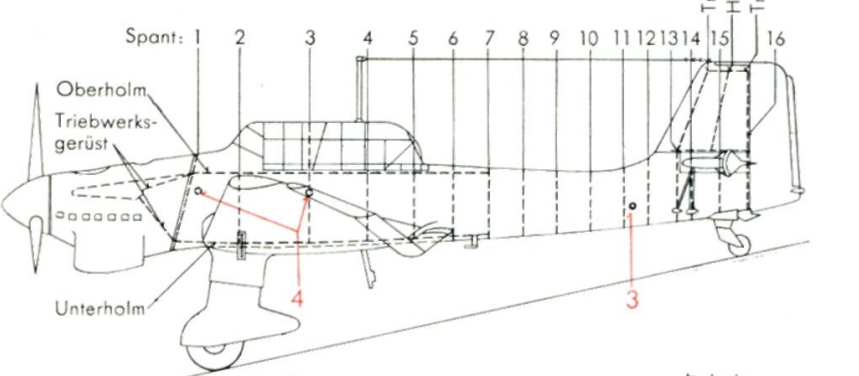
\includegraphics[width=0.75\textwidth]{media/ribbing}
  \caption{Frame or rib (German: \textit{spant}) distribution in the Stuka body \autocite{manual39}}
  \label{fig:ribs}
\end{figure}

\subsection{Wings}
The Stuka had low mounted polyhedral wings which were formed from two spars, and consisted of
three sections; a central section and a port and starboard section. The
central section was depressed to an anhedral angle of 8 degrees, while
the two other wing sections had a dihedral angle of 12
degrees. The total wingspan was 13.8m, giving a total wing area of
31.90m\textsuperscript{2}; the length of the anhedral
part of the wing on one side of the Stuka was 1.05m, while the dihedral part was
5.5m (approximate) 
\footnote{No exact values could be found for wing
  sections, so lengths were calculated based on known wingspan and cockpit
  width, and proportions from scale drawings found in Junkers manuals
  \autocite{manual39}
}
. The justification for using an inverted gull-wing
is not clear from documentation, since the polyhedral
design complicated manufacture and added weight; however, a similar wing
configuration can be found in the 1940 F4U Corsair, where the polyhedral
design allowed shorter landing gear while still providing clearance
for a 4m propeller \autocite{usni} - the Stuka's own propeller was 3.5m.
As the landing gear of the Stuka were fixed, reducing their length would reduce
drag. Another effect of the design was to cause the low
mounted wings to protrude from the fuselage at a perpendicular angle,
which would reduce interference between the wing and the body
\autocite[p~.203]{hartshorn31}. A final reason for the design could have
been to improve the pilot's visibility of the ground; the cockpit was
located above wings of the Stuka, and so the low mounting and
anhedral angle would act to remove the wings from the pilot's field of
view \autocite[p~.16]{guardia14}.

\subsection{Control Surfaces}
The Stuka used a single fin tail which had both an elevator and a
rudder for pitch and yaw control. More remarkable were the full-span ailerons
which were offset from the leading edge of the wing and operated using hydraulics. The uncommon design,
invented by Otto Maders and known as a ``Junkers flap'' \autocite{}, allowed airflow to pass
between the wing and the aileron even when the aileron was retracted.
The main effect of the flap was to ``influence the air flow around the main airfoil so
that the airfoil carried a much greater load without stalling''
\autocite[p~.14]{wenzinger38}, and in addition to reducing stall, the design
provided high lift and low drag when the Stuka was climbing. A negative
side effect was that at higher speeds the offset flap increased drag,
and therefore reduced the maximum velocity of the Stuka.

In addition to general flight properties, the ailerons could also act as
dive brakes when used with an autopilot dive bombing system. The system was engaged
by the pilot, who chose the release altitude, and would engage the ailerons at a 90 degree angle,
serving to increase drag and reduce speed while diving. The elevator
would then be adjusted down, causing the nose to drop into a dive
towards the target. At the chosen altitude, bombs would be launched from
a crutch built into the fuselage so as to avoid the propeller. Releasing
ordinance also released tension on the elevator, which was then adjusted
upwards so that the Stuka pulled out of the dive.
The system was installed after testing by Junkers showed that pullout
generated upwards of 5g of force, causing pilots to fall unconscious and
place themselves and the craft at risk.

\subsection{Materials}

The body and wings were made principally from
duralumin, an aluminum alloy composed from copper, magnesium, and
manganese
\footnote{Unfortunately, precise values for the alloy could not
  be located, but the general composition of duralumin is 93.5 - 95\% aluminum, 4\%
  copper, 0.5 - 1.0\% manganese, and 0.5 - 1.5\%
  magnesium \autocite[p.~102-103]{wardlaw33}
}, except in cases where parts were required to be more resilient to daily
wear, in which case stronger Elektron alloys were used to reduce the
need for maintenance \autocite[p.~15]{guardia14}. The outer sheeting was
also made from duralumin, and parts that underwent greater stress, such
as bolts and the canopy frame, were constructed from steel.

\subsection{Propulsion}
Thrust for the Ju 87B was provided by a variable pitch 3.5m
Jumo-Hamilton HPA III propeller which was automatically regulated, and
which was powered by a 12-cylinder Jumo 211D engine producing 883kW. The engine
was water-cooled, being fed from a 10 litre tank
\autocite[p~.7]{manual41}, and cooling was provided by two radiators
positioned above and below the engine block so that air drawn by the
propeller would pass over the radiators; this cooling action could be
controlled to some extent using cooler flaps operated by the pilot. Fuel
was injected into the engine from two 240-liter tanks, and in case of
injector failure, the gunner could hand operate a manual pump. The two
fuel tanks were located beneath the cockpit, which was protected from
the engine and tanks by an asbestos firewall. Maximum safe engine temperature
was reduced as altitude increased (Figure ~\ref{fig:temp}), limiting the
work that could be done as the Stuka climbed. Typically the Stuka
operated at 4500m, above which target sighting was impaired, and
was limited to a maximum service ceiling of 8000m due to an unpressurized cockpit.

\autocite[p~.16]{guardia14}.
\begin{figure}[h]
  \centering
  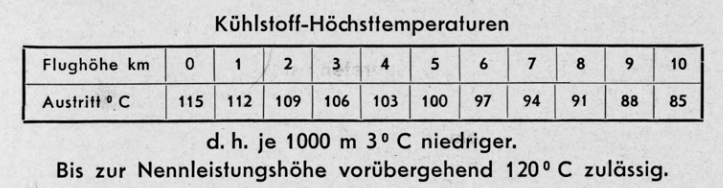
\includegraphics[width=0.75\textwidth]{media/temperature}
  \caption{Maximum temperature (in Celsius) of engine against altitude
    (in km) of Jumo 211 engine \autocite[p~.11]{manual41}}
  \label{fig:temp}
\end{figure}
The dry weight of the engine was 638kg, giving the 87B an overall unloaded
weight of 2760kg, which could be increased up to a maximum of 4400kg;
this allowed for a total possible 500kg of ordnance when accounting for
crew and fuel.
\subsection{Calculations}
\subsubsection{Lift}
For the purposes of simplification the anhedral portion of the wing is
treated as flat, since no mathematical model could be found to calculate
a polyhedral wing with anhedral and dihedral parts. Calculation is done
for temperatures of -20.7 C (Battle of Stalingrad low
\autocite[p.~731]{neumann88}) and 23.6 C (Battle of Britain
high \autocite{oxfmet}). Given these conditions, the following values
are used for calculation.
\begin{equation}\label{first}
  \setlength\tabcolsep{1cm}
  \begin{tabular}{c r}
    $L = \frac{1}{2}\ \rho V^2 S_{ref} C_L$ &
    \setlength\tabcolsep{0.2cm}
    \begin{tabular}{@{}>{$}l<{$}l@{}}
      L & Lift \\
      \rho & Density \\
      V & True Airspeed \\
      \[S_{ref}\] & Reference Area \\
      \[C_L\] & Lift Coefficient 
    \end{tabular}
  \end{tabular}
\end{equation}
\subsubsection{Drag}
\subsubsection{Speed}
\subsubsection{Range}
\section{Testing, Development, and Production}
The prototype of the 87B was the predecessor Ju 87A, which went through
a number of successive iterations during its development. The initial
design, the V1, featured a Rolls-Royce Kestrel engine and a twin
tail-fin (Figure.~\ref{fig:v1}). During a test flight the V1 crashed
when the tail could not withstand inverted flight, leading to a new V2
design with a single fin which featured in all later designs. Due to the
need for self-sufficiency in military aircraft, the British Kestrel
engine was also replaced, first by a BMW 132 engine (636 kW) in the V3, and then in the
V4 by the Junkers Jumo 210 engine.

Specific documentation on Junkers testing methods has been difficult to
find. It is likely that testing consisted of on site
factory stress testing, as well as wind-tunnel testing of models during
development, since evidence of both facilities existing can be found
\autocite{hirschel03}. Testing also consisted of a number of test
flights, likely observed by the Reichsluftfahrministerium (RLM, German
Air Ministry). Testing and development is likely to have also been
facilitated by the RLM, who took control of all German aviation after their creation
in 1933, and controlled all research from their formation to the end of
the war.

\begin{figure}[h]
  \centering
  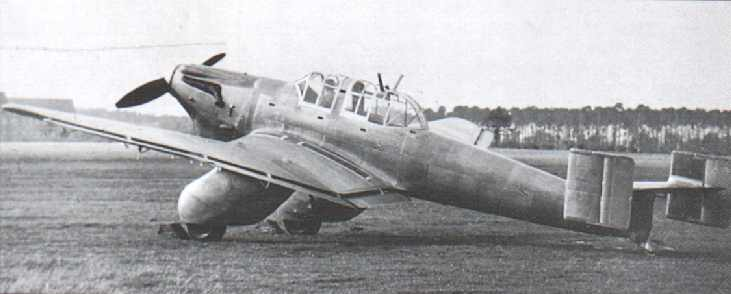
\includegraphics[width=0.75\textwidth]{media/ju87av0}
  \caption{The Ju 87A-V1 with twin tail fin and Kestrel engine
    \autocite{junkers87}}
  \label{fig:v1}
\end{figure}
\subsection{Production}
\printbibliography
\end{document}
% maximum diving speed 540 km/h \autocite[p~.56]{manual39}
